\section{塞曼效应}

\begin{quotation}
“物理学与其是被当作对先验给出的某个东西的研究,不如是被当作对给人类经验以秩序和全面考察的方法的发展。”\qquad 玻尔
\end{quotation}

塞曼效应研究磁场对光谱线的影响,原子本身可以看做是个小磁矩,或一系列小磁矩的集合。磁矩$\vec \mu$在磁场$\vec B$中的能量:

\begin{equation*}
U=-\vec \mu \cdot \vec B
\end{equation*}

取$\vec B = B \hat z$, 即磁场方向为$z$轴方向, 则:

\begin{equation*}
U=- \mu_z B
\end{equation*}

$\mu_z$就是$(\vec \mu_j)_z$,

\begin{equation*}
(\vec \mu)_z = - m_j g_j \mu_B
\end{equation*}

代入到能量的表达式中, 得到:

\begin{equation*}
U=m_j g_j \mu_B B
\end{equation*}

考虑原子中存在两个能级$E_2$, $E_1$ ($E_2 > E_1$), $B=0$时,
跃迁能量为:

\begin{equation*}
    h\nu =E_2 - E_1
\end{equation*}

如果$B \ne 0$,

\begin{eqnarray*}
% \nonumber to remove numbering (before each equation)
  E_2' &=& E_2 + m_{2}g_{2}\mu_B B \\
  E_1' &=& E_1 + m_{1}g_{1}\mu_B B
\end{eqnarray*}

能量差:

\begin{equation*}
h\nu' = E_2' - E_1' = h\nu + (m_2g_2 -m_1g_1)\mu_B B
\end{equation*}



\subsection{正常塞曼效应}

如果体系的自旋为0, 即$g_1 = g_2 =g_l =1$, 则:

\begin{equation*}
h\nu'  = h\nu + (m_2 -m_1)\mu_B B
\end{equation*}


跃迁法则:

\begin{equation*}
\Delta m = m_2 - m_1= 0, \pm 1
\end{equation*}

还有$\Delta l = \pm 1$, 谱线将分裂为三条,

\begin{figure}[h]
\begin{center}
  % Requires \usepackage{graphicx}
  \includegraphics[width=11cm]{Spectrum/normal_zeeman_effect.ps}\\
  \caption{正常塞曼效应}\label{Normal Zeeman Effect}
\end{center}
\end{figure}


\begin{equation*}
h \nu' = h\nu + \left\{ \begin{gathered}
  \mu_B B \hfill \\
  0 \hfill \\
  -\mu_B B \hfill \\
\end{gathered}  \right.
\end{equation*}


这种不需考虑自旋s, 比如两个电子形成自旋单态($S=0, 2S+1=1$),
的谱线在磁场中的分裂叫``正常塞曼效应''.


\textbf{练习1}: 试用经典物理方法导出正常塞曼效应.

解: 假设原子中电子作圆周运动, 半径为$a$, 圆频率为$\omega_0$,
向心力(centripetal force)为:

\begin{equation*}
    F_c = m_e \omega_0^2 a
\end{equation*}

加磁场B后, 会有洛仑兹力($evB = e \omega a B $)迭加于其上,
圆频率变为: $\omega = \omega_0 + \Delta$.

假设圆周运动的半径$a$不变, 这时向心力是:

\begin{equation*}
m_e \omega^2 a = F_c \pm e \omega a B
\end{equation*}

这里的$\pm$表示洛仑兹力($e v B$)的方向可能与$F_c$的方向相同,
也可能相反.

这是一个关于$\omega$的一元二次方程,

\begin{equation*}
\omega^2 \mp \frac{eB\omega}{m_e} = \frac{F_c}{m_e a}
\end{equation*}

由于: $F_c = m_e \omega_0^2 a$, 上式可化为:

\begin{equation*}
\left( \omega \mp \frac{eB}{2m_e} \right)^2 - \left(
\frac{eB}{2m_e}\right)^2 = \omega_0^2
\end{equation*}

考虑到磁场B比较小, 忽略磁场二次方项$\left(
\frac{eB}{2m_e}\right)^2$, 上式可化为:

\begin{equation*}
\left( \omega \mp \frac{eB}{2m_e} \right)^2 = \omega_0^2
\end{equation*}

即:

\begin{equation*}
\omega = \omega_0 \pm \frac{eB}{2m_e}
\end{equation*}

能量的改变是:

\begin{equation*}
 \frac{eB\hbar}{2m_e}
\end{equation*}

假设$B=1T$, 计算出$\frac{eB\hbar}{2m_e} \approx 5.8 \times 10^{-5}
eV$. 经典物理中没有量子化的概念, 所以这里其实是个能量的展宽,
即由$h\nu_0$展宽为: $h\nu_0 - \frac{eB\hbar}{2m_e} \to h\nu_0 +
\frac{eB\hbar}{2m_e}$.


\textbf{练习2}: 在氢(H), 氦(He), 锂(Li), 铍(Be), 钠(Na), 镁(Mg),
钾(K), 钙(Ca)中哪些原子会出现正常塞曼效应?为什么?

解: S=0, 意味着最外层有两个电子, 比如: He, Be, Mg, Ca.

H, Li, Na, K的最外层只有一个电子, 所以不会有正常塞曼效应.

\subsubsection{偏振特性}


\begin{figure}[h]
\begin{center}
  % Requires \usepackage{graphicx}
  \includegraphics[width=7cm]{Spectrum/momentum_of_photon.ps}\\
  \caption{光子的角动量}\label{Angular Momentum of Light}
\end{center}
\end{figure}


$\Delta m = m_2 - m_1 =1$, 原子在磁场方向(z)的角动量减少$\hbar$,
我们将观察到$\sigma^+$偏振光.

$\Delta m = m_2 - m_1 =-1$, 原子在磁场方向(z)的角动量增加$\hbar$,
我们将观察到$\sigma^-$偏振光.

对于$\sigma^{\pm}$, 电矢量在x-y平面上, 假设我们在垂直于$\vec
B$的方向上观察, 假设光沿x方向传播,
对$\sigma^{\pm}$我们将能观察到$E_y$的分量, 于是我们观察到两条与$\vec
B$垂直的``线偏振''$\sigma$光.

$\Delta m =m_2 -m_1 =0$, 原子在磁场方向(z)的角动量不变,
但由于光子本身带着角动量$\hbar$, 所以为了保证体系总的角动量守恒,
我们在平行于$\vec B$的方向观察不到$\Delta m =0$相应的$\pi$谱线,
在与磁场垂直的方向能观察到与磁场$\vec
B$平行的$\pi$谱线\footnote{详细请阅读: 杨福家《原子物理学》,
pp176;}。

\begin{figure}[h]
\begin{center}
  % Requires \usepackage{graphicx}
  \includegraphics[width=11cm]{Spectrum/zeeman_polarized.ps}\\
  \caption{塞曼效应中光的偏振特性}\label{Polarized light in Zeeman effect}
\end{center}
\end{figure}


\subsection{反常塞曼效应}

反常塞曼效应必须引入自旋概念才能解释。

我们现在来分析Na主线系双线在磁场中的分裂(即``塞曼分裂''), 即:
$3^2P_{3/2,1/2} \to 3^2S_{1/2}$. 谱线分裂将由下式决定:


\begin{equation*}
h \nu' = h \nu + (m_2 g_2 - m_1 g_1) \mu_B B
\end{equation*}


\begin{figure}[h]
\begin{center}
  % Requires \usepackage{graphicx}
  \includegraphics[width=11cm]{Spectrum/splitting_of_D_line.ps}\\
  \caption{钠D线的塞曼效应}\label{Splitting of Na D lines}
\end{center}
\end{figure}



(1)对$D_1$线, $589.6 nm$, $3^2P_{1/2} \to 3^2S_{1/2}$,

对$3^2P_{1/2}$, $g_2 = \frac{2}{3}$, $m_2=\pm \frac{1}{2}$,
$m_2g_2=\pm \frac{1}{3} $;

对$3^2S_{1/2}$, $g_1 = 2$, $m_1=\pm \frac{1}{2}$, $m_1g_1=\pm 1$;

跃迁法则: $\Delta J =0, \pm1$, 但$J=0 \nleftrightarrow J=0$,
和$\Delta M_J =0, \pm 1$.

$J=1/2 \rightarrow J=1/2$是允许的, $\Delta m = m_2 -m_1 =0$,
$\pi$线偏振光.

\begin{equation*}
h\nu' = h\nu \mp \frac{2}{3}\mu_B B
\end{equation*}


$\Delta m = m_2 - m_1 =(1/2) - (-1/2)=1$, 对应$\sigma^+$光,

\begin{equation*}
h\nu' = h\nu + \frac{4}{3}\mu_B B
\end{equation*}


$\Delta m = m_2 - m_1 =(-1/2) - (1/2)=-1$, 对应$\sigma^-$光,


\begin{equation*}
h\nu' = h\nu - \frac{4}{3}\mu_B B
\end{equation*}

即$D_1$线分裂成了四条.



(2)$D_2线$, $589.0nm$, $3^2P_{3/2} \to 3^2S_{1/2}$, 可类似考虑.

对$3^2P_{3/2}$, $g_2 =\frac{4}{3}$, $m_2=\pm \frac{1}{2}, \pm
\frac{3}{2}$, $m_2 g_2 = \pm \frac{2}{3}, \pm 2$

对$3^2S_{1/2}$, $g_1 = 2$, $m_1=\pm \frac{1}{2}$, $m_1g_1=\pm 1$;

跃迁法则: $\Delta J =0, \pm1$, 但$J=0 \nleftrightarrow J=0$,
和$\Delta M_J =0, \pm 1$.

谱线将分裂为6条。

为方便快速地画出所有正确的跃迁, 现介绍格罗春(Grotrain)图.


\begin{figure}[h]
\begin{center}
  % Requires \usepackage{graphicx}
  \includegraphics[width=6cm]{Spectrum/grotrain.ps}\\
  \caption{格罗春图}\label{Grotrain graph}
\end{center}
\end{figure}

这里向左偏的, 对应$\Delta m = m_2 -m_1=1$, 即$\sigma^+$光,
向右偏的是$\sigma^-$光, 直上直下的是$\pi$光.


\subsection{帕邢-贝克效应}

所谓``帕邢-贝克效应''(Paschen-Back effect)\index{Paschen-Back effect: 帕邢-贝克效应}就是外加磁场很强,
强到我们都可以忽略``自旋-轨道耦合''相互作用了.
因此磁矩在磁场中的能量将是:


\begin{equation*}
U = -\vec \mu \cdot \vec B = \frac{e}{2m_e}\left(g_s \vec S + g_l
\vec L \right)\cdot \vec B
\end{equation*}

取磁场方向为z轴方向, $\vec B = B \hat z$,

\begin{equation*}
U = \frac{eB}{2m_e}\left(2S_z + L_z \right) = \frac{e\hbar
B}{2m_e}\left(2m_s + m_l \right)
\end{equation*}

选择法则:

\begin{equation*}
\Delta m_s =0,  \Delta m_l =0, \pm 1, (\Delta l = \pm 1)
\end{equation*}

考虑$3P \to 3S$的跃迁, 根据选择定则将有6条跃迁,
但是只对应三个不同的能量差值, 因此只能观察到3条谱线,
其中一条与不加磁场时重叠. 在强磁场下,
``反常塞曼效应''被``帕邢---贝克效应''取代,
并趋于``正常塞曼效应的样子''.

\subsection*{习题}

\begin{enumerate}
  \item 锌原子光谱中的一条谱线(${}^3S_1 \to
  {}^3P_0$)在B为1.00T的磁场中发生塞曼分裂, 试问:
  从垂直于磁场方向观察,
  原谱线分裂为几条?相邻两谱线的波数差等于多少?是否属于正常塞曼效应?并请画出相应的能级跃迁图.
  \item 试计算在B为2.5T的磁场中, Na原子的D双线所引起的塞曼分裂.
  \item 在$B=4T$的外磁场中, 忽略自旋---轨道相互作用, 试求氢原子的$2P \to
  1S$跃迁($\lambda = 121 nm$)所产生的谱线的波长.
\end{enumerate}
